% contents

F = Festanforderung / M = Mindestanforderung / W = Wunsch

% Zellenbreite
\renewcommand{\arraystretch}{1.5}

\LTXtable{\columnwidth}{requirements_table}

\begin{table}[!h]
	\begin{tabularx}{\columnwidth}{|c|X|c|}
		\hline Erstellt durch & Kunde (Dozent) einverstanden & Version \\ 
		\hline \parbox[0pt][3em][c]{0cm}{} Team 39 &  & 1.0 \\
		\hline 
	\end{tabularx}
\end{table}	

\begin{table}[!h]
	\begin{tabularx}{\columnwidth}{|c|c|X|c|}
		\hline Version & Datum & Änderung & Verantwortlich \\ 
		\hline 1.0 & 01.10.14 & Ersterstellung & Fabian Wüthrich \\ 
		\hline 1.1 & 10.10.14 & Diverse Ergänzungen und Korrektur von Rechtschreibefehler & Fabian Wüthrich \\ 
		\hline 
	\end{tabularx}
\end{table}	

\begin{appendices}
	\chapter{Abmasse Spielfeld}\label{app:spielfeld} 
	\begin{figure}[!h]
		\centering
		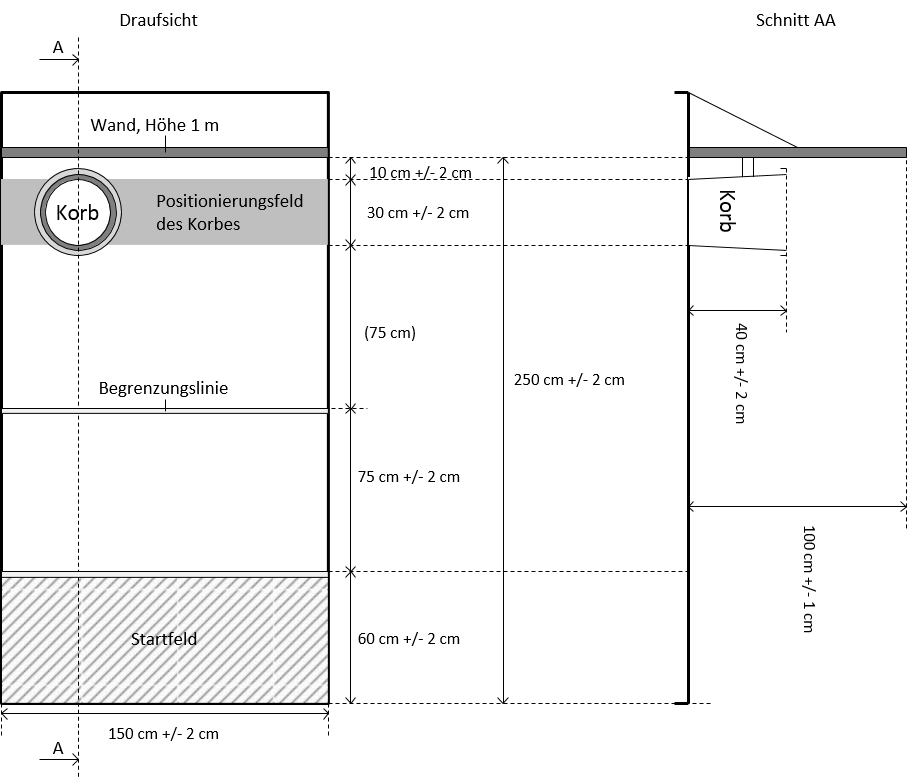
\includegraphics[width=0.7\linewidth]{../../fig/spielfeld}
		\label{fig:Bild1}
	\end{figure}
\end{appendices}